\section{Hilfsmittel Kontrollflussgraph}
Ein wichtiges Hilfsmittel ist der \textbf{Kontrollflussgraph}, der für die \textbf{Datenflussanomalieanalyse}, bestimmte \textbf{MEtriken} sowie einigen \textbf{Überdeckungskriterien} benötigt wird.

\begin{tcolorbox}[title=KOntrollflussgraph]
    \blockquote[{\cite[32, Hervorhebung eigene]{Wed09c}}]{
        Ein \textbf{Kontrollflussgraph} ist die Abbildung einer Methode auf einen gerichteten Graphen.
        Jede Anweisung entspricht einem Knoten, jeder mögliche Kontrollübergang einer Kante.
    }
\end{tcolorbox}

\subsection*{Beispiel}

Sei der folgende Sourcecode zum Zählen von großgeschriebenen Vokalen in einem Wort gegeben:

\begin{minted}{java}
    int countVowels(String txt) {
        int counter = 0;
        for (int i = 0; i < txt.length(); i++) {
            if (txt.charAt(i) == 'A' ||
            txt.charAt(i) == 'E' ||
            txt.charAt(i) == 'I' ||
            txt.charAt(i) == 'O' ||
            txt.charAt(i) == 'U') {
                counter++;
            }
        }
        return counter;
    }
\end{minted}

\noindent
Der zugehörige Kontrollflussgraph ist in Abbildung~\ref{fig:kontrollflussgraph} gezeigt.\\
Hierbei entspricht der erste Knoten der Deklaration der Definition im Kopf der Methode, die weiteren Knoten jeweils den Anweisungen.



\begin{figure}
    \centering
    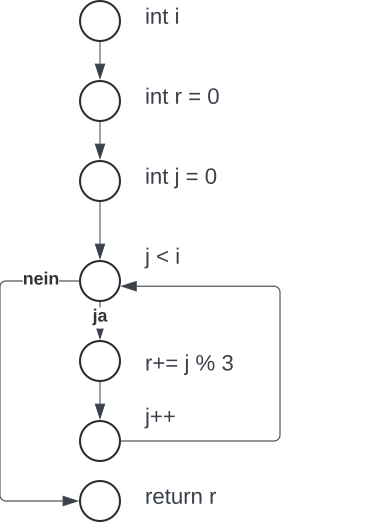
\includegraphics[scale=0.4]{part four/Werkzeuggestützte Analyse/img/kontrollflussgraph}
    \caption{Kontrollflussgraph für \textit{countVowels()}. (Quelle: in Anlehnung an \cite[Abb. 4.1, 32]{Wed09c})}
    \label{fig:kontrollflussgraph}
\end{figure}
